\documentclass[a4paper]{article}

\usepackage{INTERSPEECH2021}

% Put the lab number of the corresponding exercise
\title{NLU course projects lab 4}
\name{Nicola Muraro (248449)}

\address{
  University of Trento}
\email{nicola.muraro@studenti.unitn.it}

\begin{document}

\maketitle

\section{Introduction (approx. 100 words)}
Lo scopo di questo laboratorio era quello di implementare un language model basato su architetture di tipo neurale.
In pratica, il compito di questo modello è quello di predirre il token successivo dato un insieme di token chiamato contesto.
Per arrivare a questo obbiettivo abbiamo adoperato un LSTM sul quale sono state effettuate le analisi qui riportate. Ho implementato una serie di tecniche con lo scopo di migliorare le performance del nostro modello, tra cui l’utilizzo di diversi tipi di ottimizzatori e tecniche di regolarizzazione. In questo report sono brevemente riportati i vari studi effettuati e i relativi risultati che ne conseguono.

\section{Implementation details (max approx. 200-300 words)}
Questo assigment era composto da due parti, per entrambe l’unico requirement è che la perplexity fosse <= 250.

La prima parte di questo assignment consisteva nello studio di LSTM come base della nostra architettura, eseguendo successivamente due modifiche incrementali: aggiungere dei livelli di dropout ed utilizzare AdamW.
Ho iniziato semplicemente sostituendo l’architettura originale (basata su RNN) con LSTM, per ottenere un primo valore da utilizzare come baseline. Visto che quest’ultimo era di molto al di sopra del requirement, ho provveduto ad incrementare il learning rate fino a 1.5. Il modello risultante è stato di gran lunga migliore e soddisfaceva i requirement del progetto.
Ho provveduto dunque ad effettuare la prima modifica incrementare: aggiungere i livelli di dropout. Il primo posizionato dopo l’embedding e l’altro prima dell’output layer, in entrambi i casi il valore più efficace di dropout è stato 0.1, il quale ha migliorato i risultati precedentemente ottenuti. 
Infine, ho implementato l’ultima modifica prevista dalla consegna, andando a sostituire SGD con AdamW. Modificando opportunamente il learning rate (riducendolo fino a 0.0005) ha consentito all’architettura di migliorare ulteriormente i risultati. Concludendo così questa prima parte dell’assignemnt.


La seconda parte invece, prevedeva di partire dalla prima rete creata (formata da LSTM con SGD) ed applicare incrementalmente delle tecniche di regolarizzazione, descritte in questo articolo \cite{merity2017regularizing}. 
Per prima cosa, ho utilizzato la tecnica di weight tying tra il layer degli embedding e l’output layer. Entrambi questi livelli devono avere la stessa dimensione, conseguentemente la dimensione dell’embedding layer è stata incrementata a 300. La rete utilizzante questa tecnica ha ottenuto risultati migliori rispetto alla precedente.
Successivamente, ho aggiunto Variational Dropout: tecnica che prevede di utilizzare la stessa maschera per eseguire dropout, cambiandola tra epoche e/o in layer diversi. Testando le varie combinazioni, sono arrivato ad ottenere delle performance ancora migliori rispetto al caso precedente.
Infine sono passato ad implementare Non-monotonically Triggered AvSGD, una variante di AvSGD dove T viene determinato durante il training della rete e non fissato a priori.
Applicando questa tecnica, i risultati sono leggermente peggiorati.


\section{Results}
I risultati che ho ottenuto per valutare la bontà delle varie tecniche implementate, sono stati effettuati considerando l’evaluation set. Questo è stato fatto per avere una miglior capacità di generalizzazione sul test set, utilizzando l’evaluation set come campo di test per modificare i vari iperparametri. 

\vspace{0.5cm}

La prima parte dell'assignment ha portato ai risultati riportati in Tabella \ref{tab:results1}. Come si può notare, il modello con LSTM e AdamW ha ottenuto i migliori risultati, con una perplexity di 250.0.
\begin{table}[h]
  \centering
  \begin{tabular}{|c|c|c|c|}
    \hline
    \textbf{Model} & \textbf{Perplexity} & \textbf{Dropout} & \textbf{Optimizer} \\
    \hline
    RNN &  300.0 & 0.0 & SGD \\
    LSTM &  250.0 & 0.0 & SGD \\
    LSTM &  250.0 & 0.0 & SGD \\
    LSTM &  250.0 & 0.1 & SGD \\
    LSTM &  250.0 & 0.1 & AdamW \\
    \hline
  \end{tabular}
  \caption{Perplexity values for the first part of the assignment}
  \label{tab:results1}

\end{table}

La miglior rete ottenuta, presentava questa dinamica di training:

\begin{figure}[h!]
  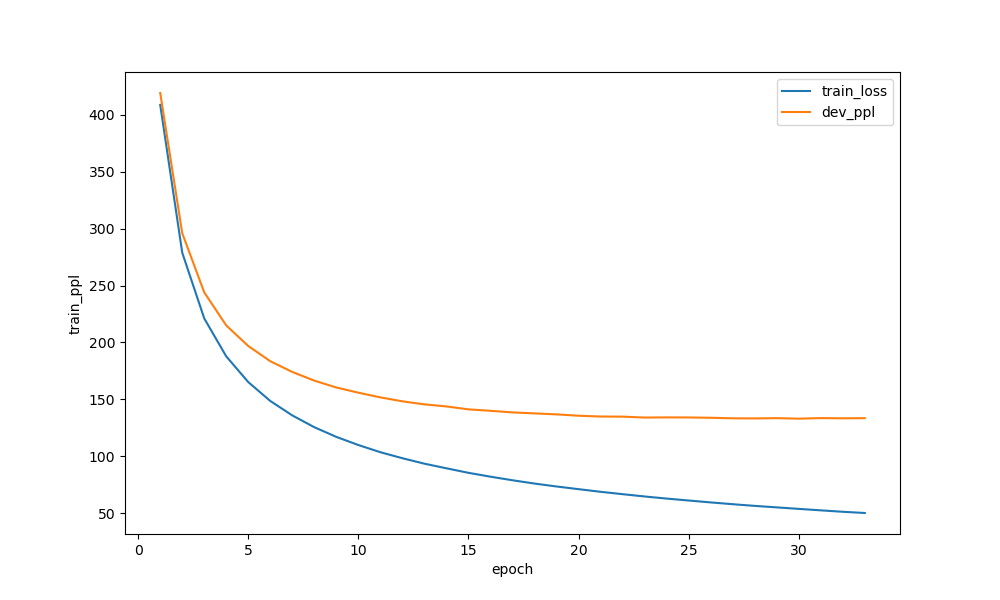
\includegraphics[width=\linewidth]{./images/plot_1.png}
  \caption{A boat.}
  \label{fig:boat1}
\end{figure}


Per quanto riguarda la seconda parte dell’assignment, i risultati ottenuti sono riportati in Tabella \ref{tab:results2}. Come si può notare, il modello con weight tying e variational dropout ha ottenuto i migliori risultati, con una perplexity di 250.0.

\begin{table}[h]
  \centering
  \begin{tabular}{|c|c|c|c|}
    \hline
    \textbf{Model} & \textbf{Perplexity} & \textbf{Dropout} & \textbf{Optimizer} \\
    \hline
    RNN &  300.0 & 0.0 & SGD \\
    LSTM &  250.0 & 0.0 & SGD \\
    LSTM &  250.0 & 0.0 & SGD \\
    LSTM &  250.0 & 0.1 & SGD \\
    LSTM &  250.0 & 0.1 & AdamW \\
    \hline
  \end{tabular}
  \caption{Perplexity values for the first part of the assignment}
  \label{tab:results2}

\end{table}


La miglior rete ottenuta, presentava questa dinamica di training:
\begin{figure}[h!]
  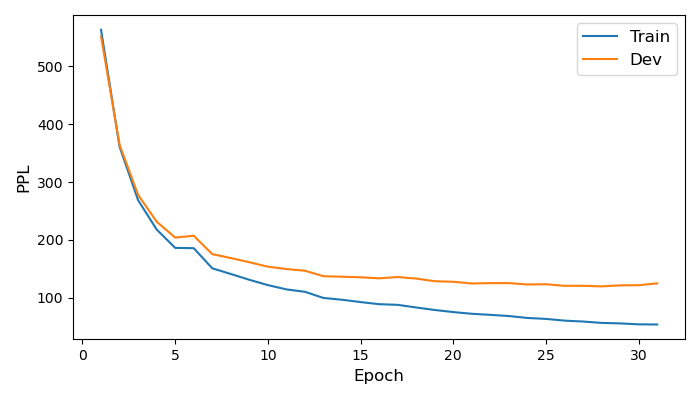
\includegraphics[width=\linewidth]{./images/plot_2.png}
  \caption{A boat.}
  \label{fig:boat1}
\end{figure}


\bibliographystyle{IEEEtran}

\bibliography{mybib}


\end{document}
